\chapter{Implementation}
\label{ch:implementation}

\section{Implementation of the mod}

\begin{figure}[H]
\centering
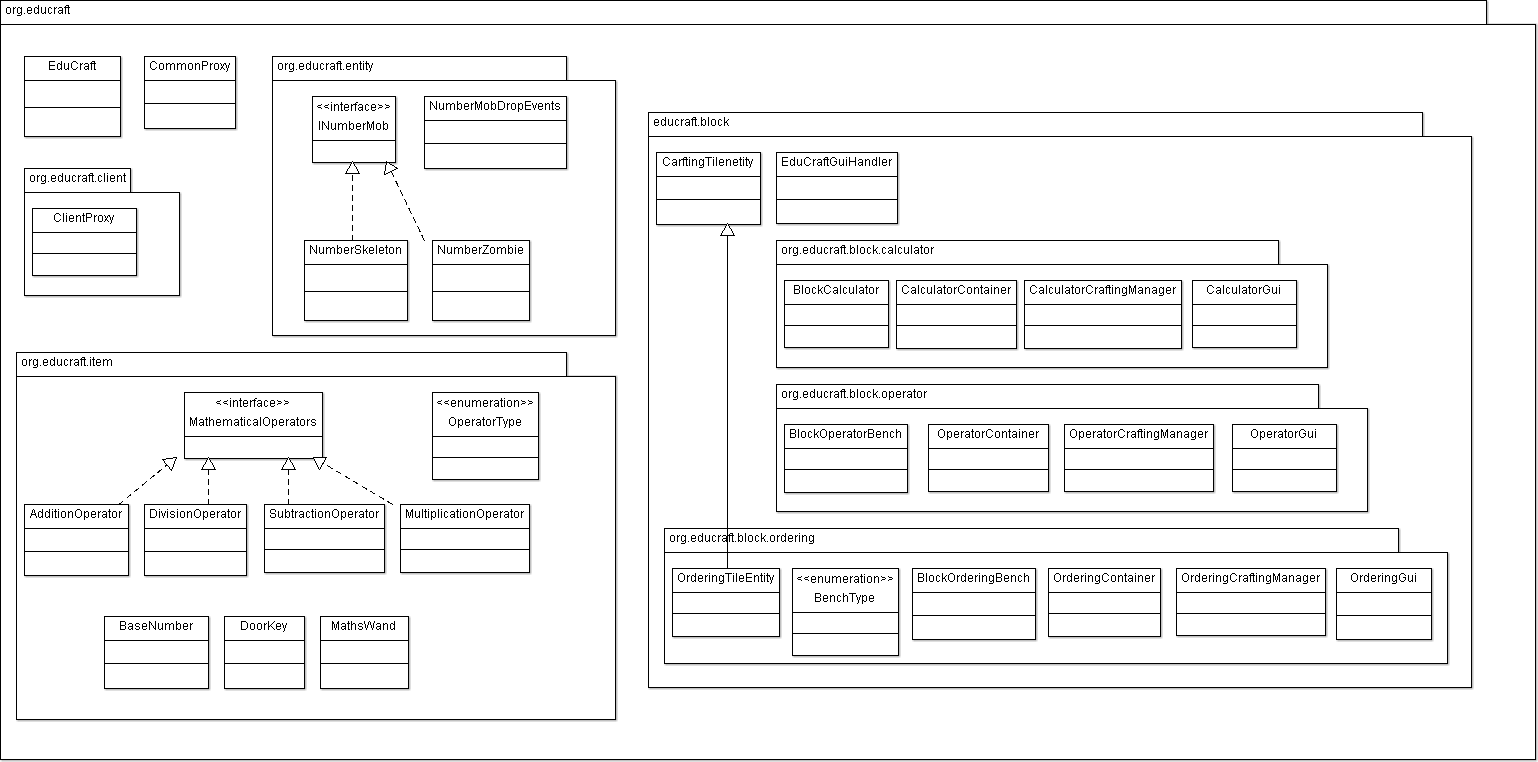
\includegraphics[width=17cm, height=11cm]{ClassDiagram}
\caption{"UML class diagram of EduCraft"}
\end{figure}

\begin{itemize}
\item \textbf{Base Mod Class}\footnote{``The base class is the class that Forge loads. All the classes in our mod have to be registered through this central location for the mod. It is advised to name this class after the name of the Mod. In our case it is EduCraft''\cite{website:forge-basemods}}\newline
The Base Mod needs to contain the following line:
\begin{lstlisting}
@SidedProxy(clientSide="tutorial.generic.client.ClientProxy",serverSide="tutorial.generic.CommonProxy")
public static CommonProxy proxy;
\end{lstlisting}

\item \textbf{Proxy Classes}\footnote{``Minecraft uses a client and server setup even on single player. The server side does all the maintaining of the world’s state while the client render’s the world. All code runs on both sides unless specified otherwise.\newline
The annotation @SidedProxy is used when we want the server to call the constructor of one class and the client the other. We use the proxy for registering images and hosting our GUI handler.\cite{website:forge-proxy}}
\end{itemize}

\section{Implementation of Constraints}

\section{Implementation of Items}

\section{Implementation of Blocks}
This section covers the most important steps that allowed us to create our own Crafting Tables with custom looks and specific behaviours.\newline\newline
During our initial attempts to create a modified Crafting Table we came across the problem of implementing our Numbers efficiently. We initially thought that we would have to hardcode every single class for each Number item that could be used in the Calculator without having to create separate recipes. This stalled our progress for while, but luckily after a substantial amount of research we found a solution. This workaround allowed us to have one BaseNumber class and every time a new BaseNumber object is created a random metadata is assigned to that specific item. The metadata defines the value, the texture used and the onscreen text displayed for that Number item. After this issue was resolved we were able to proceed with the implementation of the Calculator.\newline\newline
Minecraft distinguishes between two different ways of handling information due to being a multiplayer game, we will refer to these as Server Side and Client Side. The original Crafting Table only opens on the Client Side, which limits the interaction with this object to one player at a time. Initially we started with an implementation that only added custom looks and behaviours to our Crafting Tables. Later on, we recognised the importance of making the Crafting Tables Server Side to allow multiple players to interact with the same block simultaneously. This helped us to create an even more collaborative gaming experience.

\subsection{Chain of method calls during the use of Crafting Table}

\subsection{Extended Block Types}
The Ordering Table has three different types depending on the parity of the input numbers accepted by it. We have created an enum type named BenchType to describe the different types of Ordering Tables. OrderingTileEntity classes are created with an additional field differentiating the specific Ordering Table in the world when the block is created. This attribute will determine the behaviour of the Ordering Tables based on their type.

\subsection{CraftingTileEntity}
We created this class subsequent to our findings relating to the use of the Chest by multiple players simultaneously. We investigated how the Chest worked and found that Tile Entities are used to implement this feature.\newline
Tile Entities are bound to specific coordinates in the world and their fields hold unique values. In the case of the Crafting Table, they hold the inventory of a Block. This allows interaction that can be seen by everyone over the network.\newline
An additional field in our version of the Tile Entities keeps track of the number of players using the Block.\newline
The default constructor is not capable of setting up a crafting matrix (collection of input slots) as the CraftingTileEntity does not have a reference to a container on creation. Our work around was to initialise the CraftingTileEntity as soon as we create a container for a Block.\newline
\begin{lstlisting}
public synchronized CraftingTileEntity initialise(Container container) {
	if (this.container == null) {
		this.container = container;
this.craftMatrix = new InventoryCrafting(this.container, 1, 3);
		this.craftResult = new InventoryCraftResult();
	}
	incrUsers();
	return this;
}
\end{lstlisting}

\subsection{GuiHandler}
This class is essential for handling our custom-made GUIs. It implements the core IGuiHandler interface and has two methods:
\begin{itemize}
\item getServerGuiElement(...)\newline
generates a container, which forms the Server Side of The GUI
\item getClientGuiElement(...)\newline
generates the GUI itself, which is displayed in the Client Side
\end{itemize}

\subsection[Container]{Container\footnote{``The container is what connects the inventories of the player and tileentity to the GUI. The constructor defines the position on-screen and contents of each slot.''\cite{website:forge-container}}}
The following are the changes we made to our extended version of the container to create a custom layout of the slot matrix:
\begin{itemize}

\item in the case of a Client Side only Crafting Table, field in class:
\begin{lstlisting}
public InventoryCrafting craftMatrix = new InventoryCrafting(this, x, y);
\end{lstlisting}

\item in the case of a Server Side Crafting Table, in constructor:
\begin{lstlisting}
this.tileEntity = tileEntity.initialise(this, x, y);
\end{lstlisting}

\let\thefootnote\relax\footnote{x = the number of rows}
\let\thefootnote\relax\footnote{y = the number of columns}

\item in any case, in constructor:
\begin{lstlisting}
// adds output slot to the container
this.addSlotToContainer(new SlotCrafting(inventory.player,	this.craftMatrix, this.craftResult, 0, 124, 35));
			
	// adds input slots to the container
	for (int l = 0; l < x; ++l) {
		for (int i1 = 0; i1 < y; ++i1) {
			this.addSlotToContainer(new Slot(this.craftMatrix, i1 + l * 3, 30 + i1 * 18, 17 + l * 18));
		}
	}
\end{lstlisting}

\let\thefootnote\relax\footnote{x = the number of rows}
\let\thefootnote\relax\footnote{y = the number of columns}
\let\thefootnote\relax\footnote{Please note that in Slot(..., x, y, z) and SlotCrafting(..., x, y, z) the last three arguments passed in are slotIndex, xDisplayPosition and yDisplayPosition in this order. Coordinates are represented in pixels. The default size of a slot is 18x18 pixels.}

\item in the case of a Server Side Crafting Table, in the onContainerClosed() method:	
\begin{lstlisting}
/**
 * Called whenever the container is closed. If no one is using the container
 * any more, then it should drop everything inside it, like a crafting
 * table.
 * 
 * @param player
 *            the player who closed the container
 */
@Override
public void onContainerClosed(EntityPlayer player) {
	super.onContainerClosed(player);
	this.tileEntity.decrUsers();

	if (!this.worldObj.isRemote && !this.tileEntity.isBeingUsed()) {
			for (int i = 0; i < 3; ++i) {
				ItemStack itemstack = this.craftMatrix.getStackInSlotOnClosing(i);
            
				if (itemstack != null) {
					player.dropPlayerItem(itemstack;
				}
			}
	}
}
\end{lstlisting}
\end{itemize}

\subsection{Gui}
This class is responsible for the creation and display of GUIs.
There are two methods within this class. One is responsible for drawing the background and the other one is for drawing the foreground.\newline\newline
\begin{lstlisting}
/**
* Standard prefix for every GUI texture created for the mod.
*/
public static final String GuiTexturePrefix = "educraft" + ":" + "textures/gui/";

private ResourceLocation calculator = new ResourceLocation(EduCraft.GuiTexturePrefix+ "FileName.png");
\end{lstlisting}

\subsection{CraftingManager}
In the Crafting Manager classes for the Calculator and Ordering Bench we simplified the operation of the core version of this class. This was possible as we are not using any Recipes for implementing the logic of how the inputs are checked and the way the output is generated. Both Crafting Tables have only 3 input slots and this allowed us to validate inputs in a simpler manner.\newline\newline
The logic implemented for the Calculator is to have two operands (instance of BaseNumber) in slots 1 and 3 and an operator (instance of MathematicalOperator) in slot 2 of the input matrix. If this condition is not met then there is nothing to generate or else it gets the metadata value (itemDamage) of the operands and the mod internally performs a mathematical operation depending on the type of operator. An output BaseNumber is generated, with the result of the operation stored in the new items metadata. There are a few cases where there is nothing generated even though the operation would be mathematically correct, but our mod does not cover the use of negative numbers, fractions and decimals. We would like to implement these concepts in future versions of the extension.\newline\newline
\begin{figure}[H]
\centering
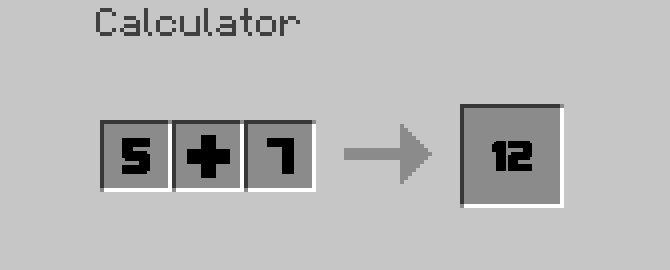
\includegraphics[scale=0.4]{calculator_use_top}
\caption{Screenshot of the Calculator's crafting matrix in use}
\end{figure}

The Crafting Manager for the Ordering Bench works in a similar way, but it first tests if all the inputs are numbers and then it checks if the order and the parity of the numbers are valid depending on the type of the Ordering Table and finally it generates a coloured key.\newline\newline
\begin{figure}[H]
\centering
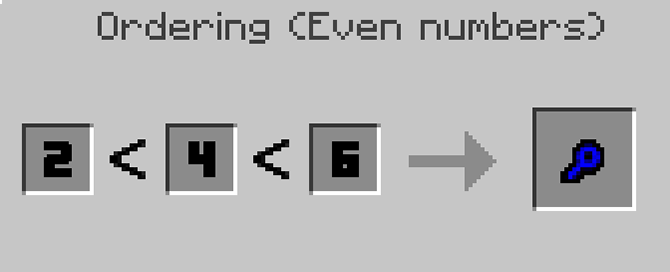
\includegraphics[scale=0.4]{ordering_use_top}
\caption{Screenshot of the Ordering Bench's crafting matrix in use}
\end{figure}

We decided to keep the way the core Crafting Manager works for the Operator Bench. This bench has the same behaviour as the core Crafting Table. The only modifications are the visuals and the recipes accepted. We wanted to limit the items that could be crafted by the players in the mod. We achieved this by placing only our own modified versions of the Crafting Tables in our levels. These benches accept only our custom recipes which we defined for the crafting \footnote{``Crafting is the method by which many blocks, tools, and materials are made in Minecraft. In order to craft something, players must move items from their inventory to a crafting grid. A 2×2 crafting grid can be accessed from the player's inventory. A 3×3 grid can be accessed by right-clicking a Crafting Table.''} of the mathematical operators. All these recipes are ShapedRecipes\footnote{``Shaped recipes come in all sizes from 1x1 to 3x3. Strings are used for the recipe shape and values.''\cite{website:forge-shaped}} used in the original version of Minecraft.
\begin{figure}[H]
\centering
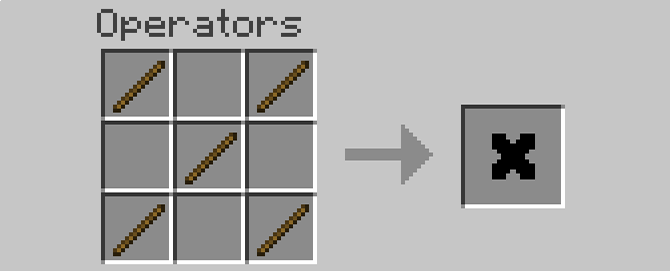
\includegraphics[scale=0.4]{operator_use_top}
\caption{Screenshot of the Operator Bench's crafting matrix in use}
\end{figure}
The method signature is roughly as follows:
\begin{lstlisting}
this.addRecipe(String row1, [String row2[, String row3]]
        char itemType1, ItemStack itemStackType1[, ... char itemTypeN, ItemStack itemStackTypeN]);
\end{lstlisting}
A list of all the recipes added to the Operator Bench:
\begin{lstlisting}
/** A list of all the recipes added */
private List<IRecipe> recipes = new ArrayList<IRecipe>();

private OperatorCraftingManager() {
	ItemStack sticks = new ItemStack(Item.stick);
	this.addRecipe(new ItemStack(EduCraft.ADD_OPR), " s ", "sss", " s ", 's', sticks);
	this.addRecipe(new ItemStack(EduCraft.SUB_OPR), "   ", "sss", "   ", 's', sticks);		this.addRecipe(new ItemStack(EduCraft.MUL_OPR), "s s", " s ", "s s", 's', sticks);
	this.addRecipe(new ItemStack(EduCraft.DIV_OPR), "  s", " s ", "s  ",'s', sticks);
}
\end{lstlisting}

\section{Implementation of Mobs}
\section{Implementation of Locations}
We used creative mode\footnote{``Creative mode is one of the main game modes in Minecraft. This mode strips away the survival aspects of Minecraft and allows players to easily create and destroy structures. Creative mode allows players to destroy all blocks instantly (including normally-indestructible blocks such as bedrock) and the ability to fly. Players are given an infinite number of blocks to build with and no health or hunger bar thus rendering the player immune to all damage.''\cite{website:minecraft-creative}} in Minecraft to create all the different locations (levels) in our world. In order to make the visual experience in the mod more enjoyable we used a world editing tool called MCEdit to create a small forest and mountains in the surrounding area of the locations.
We have also created our own tab for easier access of custom elements in the inventory list. We added the following line to the constructors of all elements created by us:
\begin{lstlisting}
setCreativeTab(EduCraft.tabEduCraft);
\end{lstlisting}
\begin{figure}[h!]
\centering
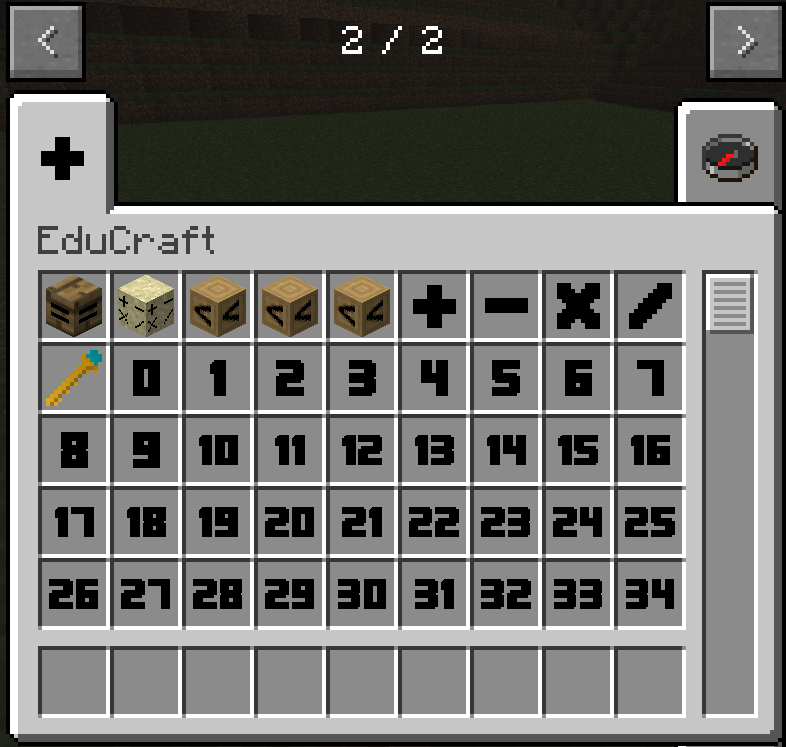
\includegraphics[scale=0.4]{educraft_tab}
\caption{"Screenshot of EduCraft custom tab in game inventory"}
\end{figure}

\subsection{Castle}
The collaborative element of this level was implemented by setting a task to create four different operators, which would open doors to four different rooms using the hopper system in the first part of the level. Each room has a key inside and all four keys are needed to allow the players to progress to the next part of this level.\newline\newline
In the next part each player will have to pick up a Maths Wand and kill some Zombies and collect enough numbers to be able to use the Ordering Bench. A correct ordering of numbers will generate a key that opens the door leading to the final part of this level.\newline\newline
In the final part the team has to obtain a specific number through a series of mathematical operations to be able to leave the level through the exit. There is a chest full of Mathematical Operators which they can use within the Calculator. The team has to kill Zombies and Skeletons to collect the numbers dropped by the monsters.\newline\newline
All tasks in this part are designed so no one can progress without the help of the others. This was set to be a tutorial level which would allow the players to familiarise themselves with the game play of the mod.
\subsection{Pyramid}
This level forces the team to split up at the beginning. This is achieved by only allowing two players inside the Pyramid. As soon as there are two players inside the entrance is blocked.\newline\newline
The interior of the Pyramid has two floors and it is divided into four sections. The Pyramid is surrounded by a garden with fences and walls so as to prevent the outside team from wandering around in the world. Each inner section has its own corresponding outer garden section. Neither the inside nor the outside team can go to the next section without collaboratively working towards a goal set for each section of the level.\newline\newline
There is an exit through the top of the Pyramid for the inside team. The inside team can only leave once each subteam has generated a key in the fourth section of the level. The outside team can climb the stairs on the side of the Pyramid in the fourth section and throw their key inside for the other team. The inside team should have two keys by this point and each key will move a block, creating a path to leave. Once all the players are reunited, they can leave through the level exit, which located in the final garden section.\newline\newline
In each section the resources available are limited for each subteam, for example in one section the inside team has access to sticks and an Operator Bench, but not to any numbers. In the same section the outside team has the opportunity to kill Zombies or Skeletons to be able to collect numbers and they also have a Calculator to generate numbers.\newline\newline
We implemented a system that allows the teams to send items back and forth in minecarts that move on rails. This will force them to communicate their requirements to each other.\newline

\begin{figure}[h!]
\centering
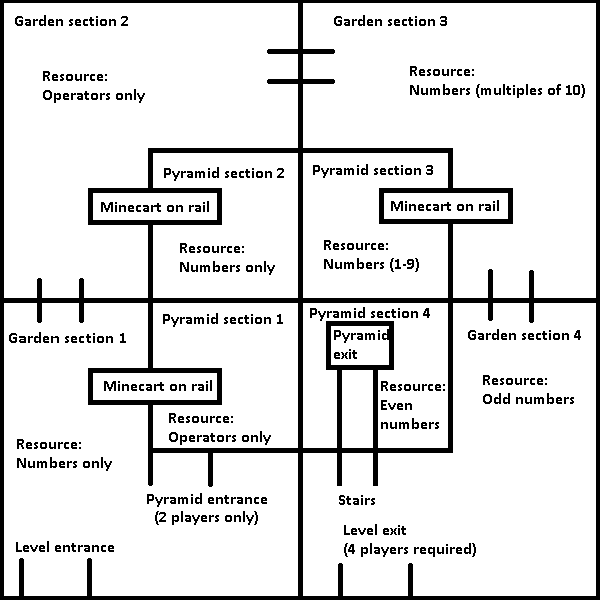
\includegraphics[scale=0.65]{pyramid}
\caption{Sketch of the Pyramid's layout}
\end{figure}

\subsection{Rook}
The Rook has two floors and on each floor there are two rooms. Only the first two players to arrive can enter each room. The subteams’ resources are limited in a similar manner to the Pyramid. The rooms on the same floors share a wall. In each of these walls there is a Calculator built-in, which can be used by the subteams to pass items to each other and to execute some mathematical operations together.\newline\newline
In order to leave the rooms the teams must generate a specific number and throw that number in the hopper by the exit. Each exit is connected to a staircase that leads to the floor above. The “roof top” of the Rook is the final destination in our game. It is relatively elevated, so the players can have a look around and see the world and all the levels they have completed.


